\section{\Naive\ parameter inference via Metropolis-Hastings}

The key idea of the dependent-thinning approach of~\cite{RaoTeh13} is
to introduce a set of thinned candidate transition times $U$ from
a rate-$(\Omega-A_{S(t)})$ Poisson process. These, along 
with the extant transition times $T$, form a random grid $W$, conditioning on
which sampling a new trajectory reduces to a standard discrete-time 
HMM sampling step. This suggests conditioning on the random grid to update
the MJP parameters according to the discrete-time MH-scheme from
algorithm~\ref{alg:disc_time_mh}.
%The resulting scheme updates $\theta$ conditioned on the random 
%grid, but with the trajectory integrated out 
In particular, we propose a new parameter $\theta^*$ from $q(\theta^*|\theta)$, 
now conditioning on the set of times $W$.
We then make a forward pass over $W$, and calculate
the marginal probabilities $p(X|W,\theta)$ and $p(X|W,\theta^*)$. These can be
used to calculate the MH-acceptance probability $\min\left(1,
\frac{p(X|W,\theta^*)p(W|\theta^*)p(\theta^*)q(\theta|\theta^*)}
     {p(X|W,\theta)p(W|\theta)p(\theta)q(\theta^*|\theta)}\right)$. 
After accepting or rejecting $\theta^*$, the new $\theta$ can be used in
a backward pass that samples a new trajectory. We then discard all 
self-transitions and repeat; figure~\ref{fig:naive_mh} sketches out the resulting
scheme.

The resulting scheme updates $\theta$ with the MJP trajectory integrated out, 
and one would expect it to mix more rapidly that Gibbs sampling. 
It is important to note however that $\theta$ is updated conditioned on
$W$, and that
%determines not just the MJP trajectory $S(t)$.
%, and with $S(t)$ 
%marginalized out, the observations $X$. 
the distribution of $W$ depends on $\theta$. These are the $p(W|\theta)$ terms
in the acceptance probability; under uniformization, $W$ follows a homogeneous
Poisson process with rate $\Omega(\theta) = 2 \max A(\theta)$. 
%who probability can
%calculated easily during the forward pass.
The fact that the MH-acceptance probability involves a $p(X|\theta)$ term
is inevitable, however in our experiments, we found that the $p(W|\theta)$
terms have a significant effect acceptance probability. 
Any proposal that halves $\max A_s$ (and thus $\Omega$) will halve the
mean and variance of the distribution of the number of events in $W$, 
resulting in an extremely low acceptance probability.
In the next section, we describe a way around this issue.
\setlength{\unitlength}{0.8cm}
  \begin{figure}[H]
  \centering
  \begin{minipage}[!hp]{0.45\linewidth}
  \centering
    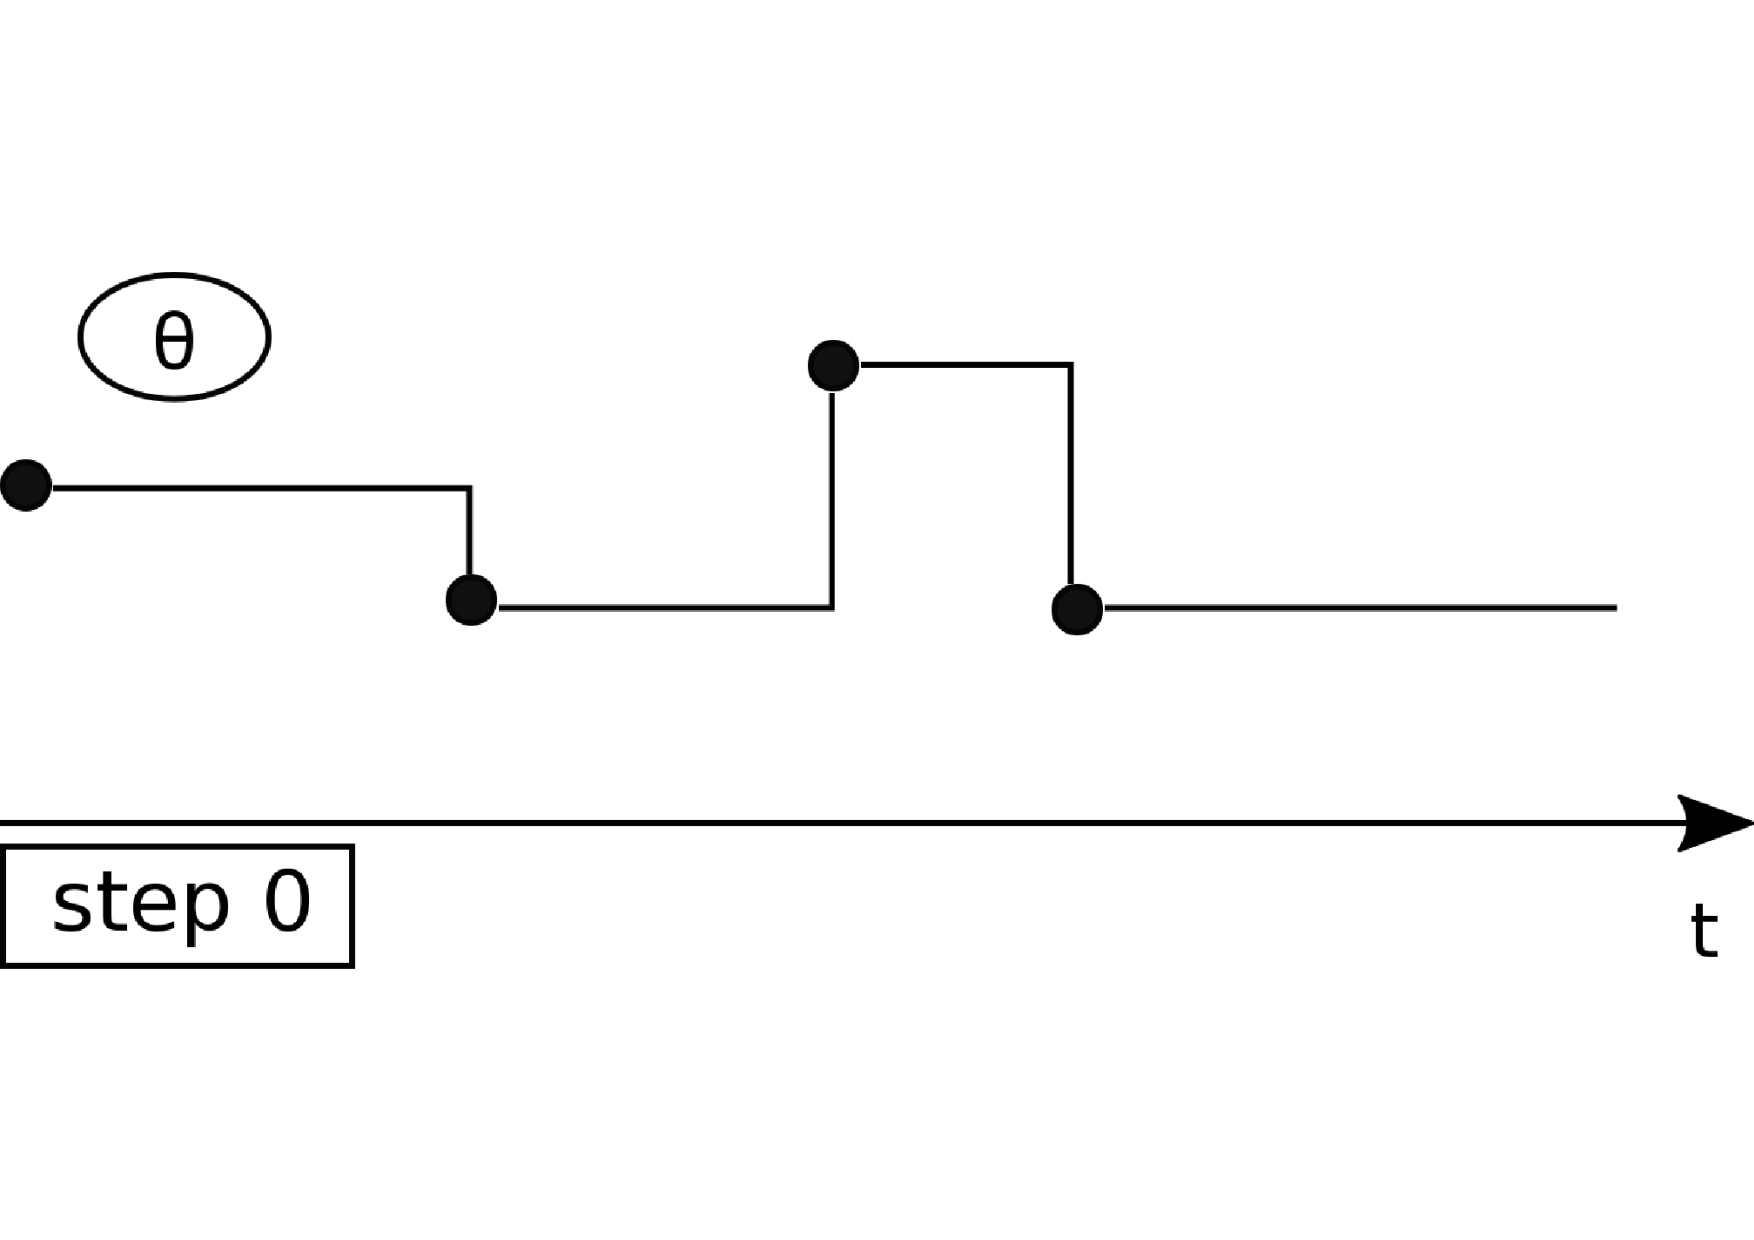
\includegraphics [width=0.70\textwidth, angle=0]{figs/plotn0.pdf}
      \end{minipage}
  \begin{minipage}[!hp]{0.45\linewidth}
  \centering
    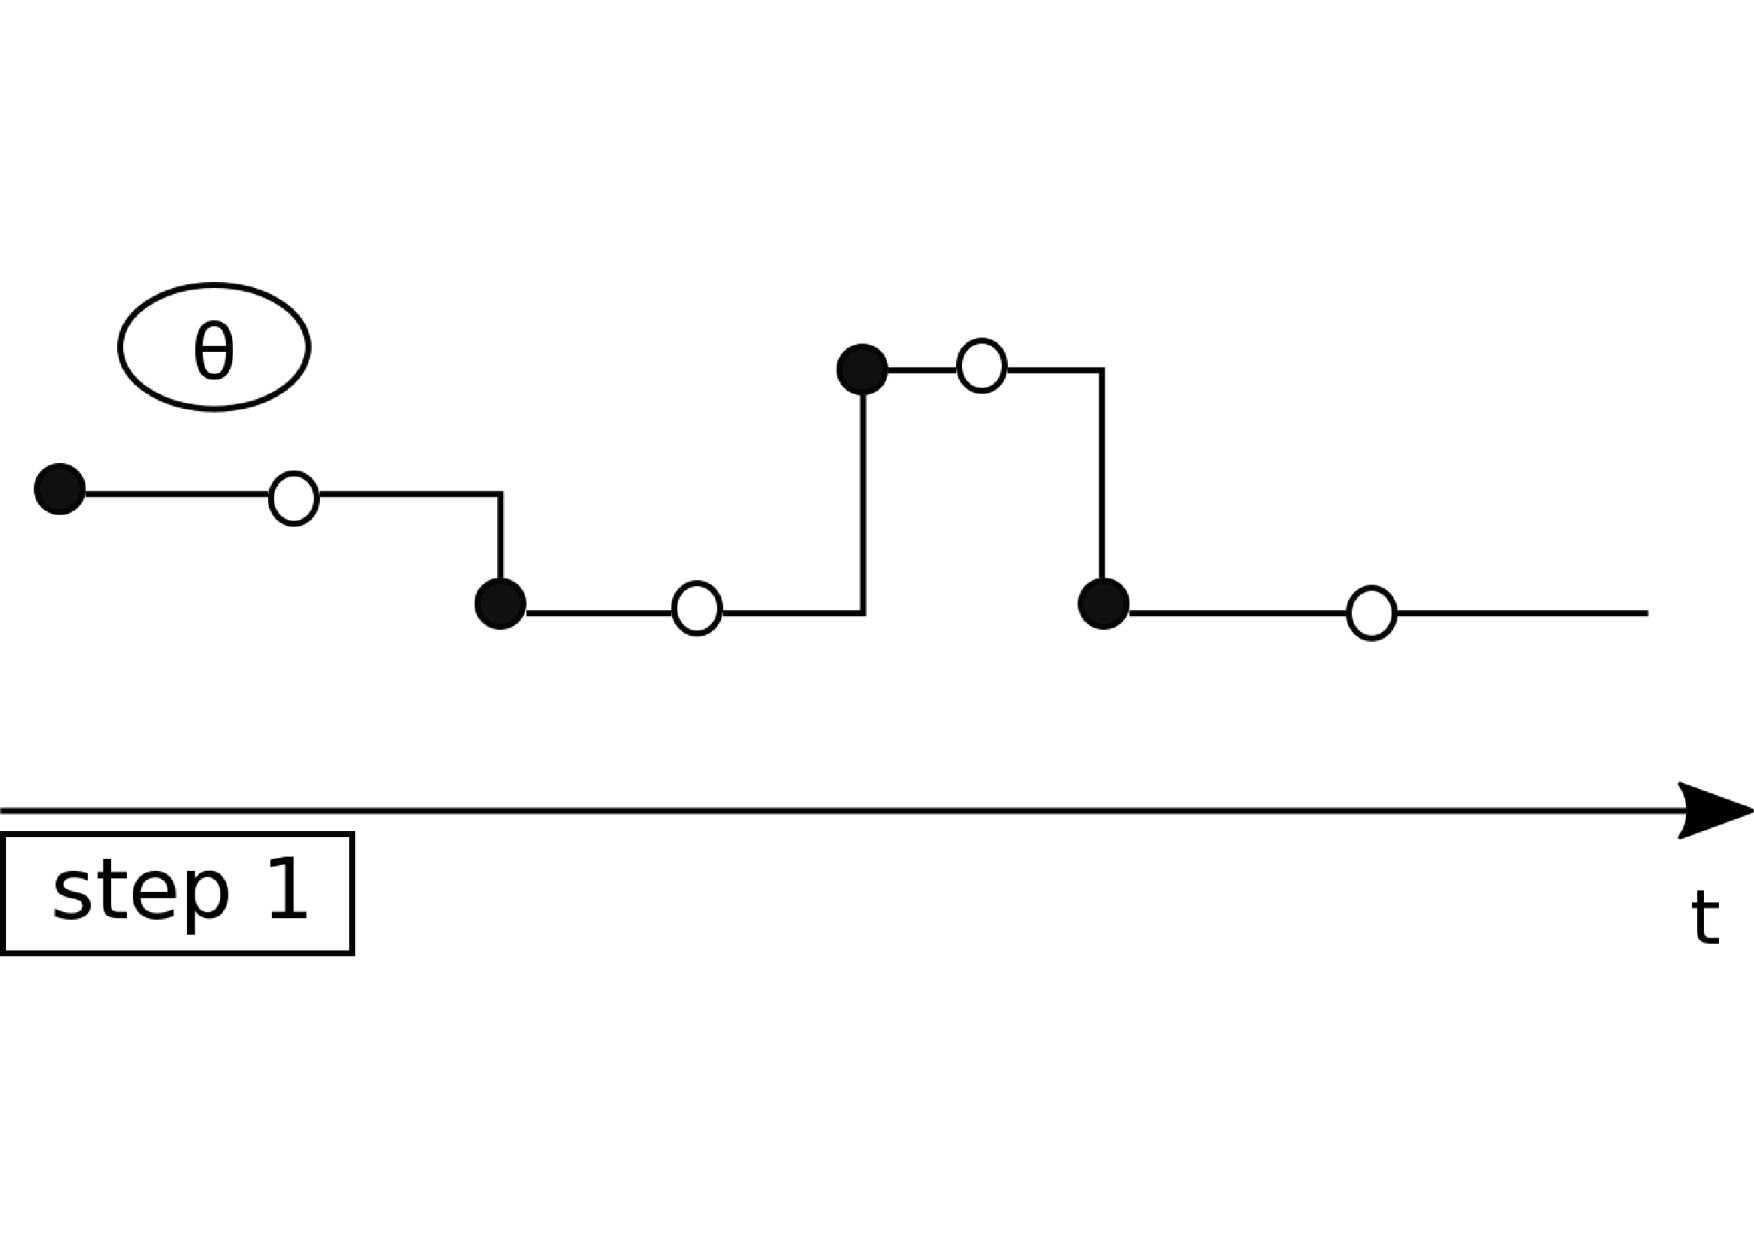
\includegraphics [width=0.70\textwidth, angle=0]{figs/plotn1.pdf}
    \vspace{-0 in}
  \end{minipage}
  \begin{minipage}[!hp]{0.45\linewidth}
  \centering
    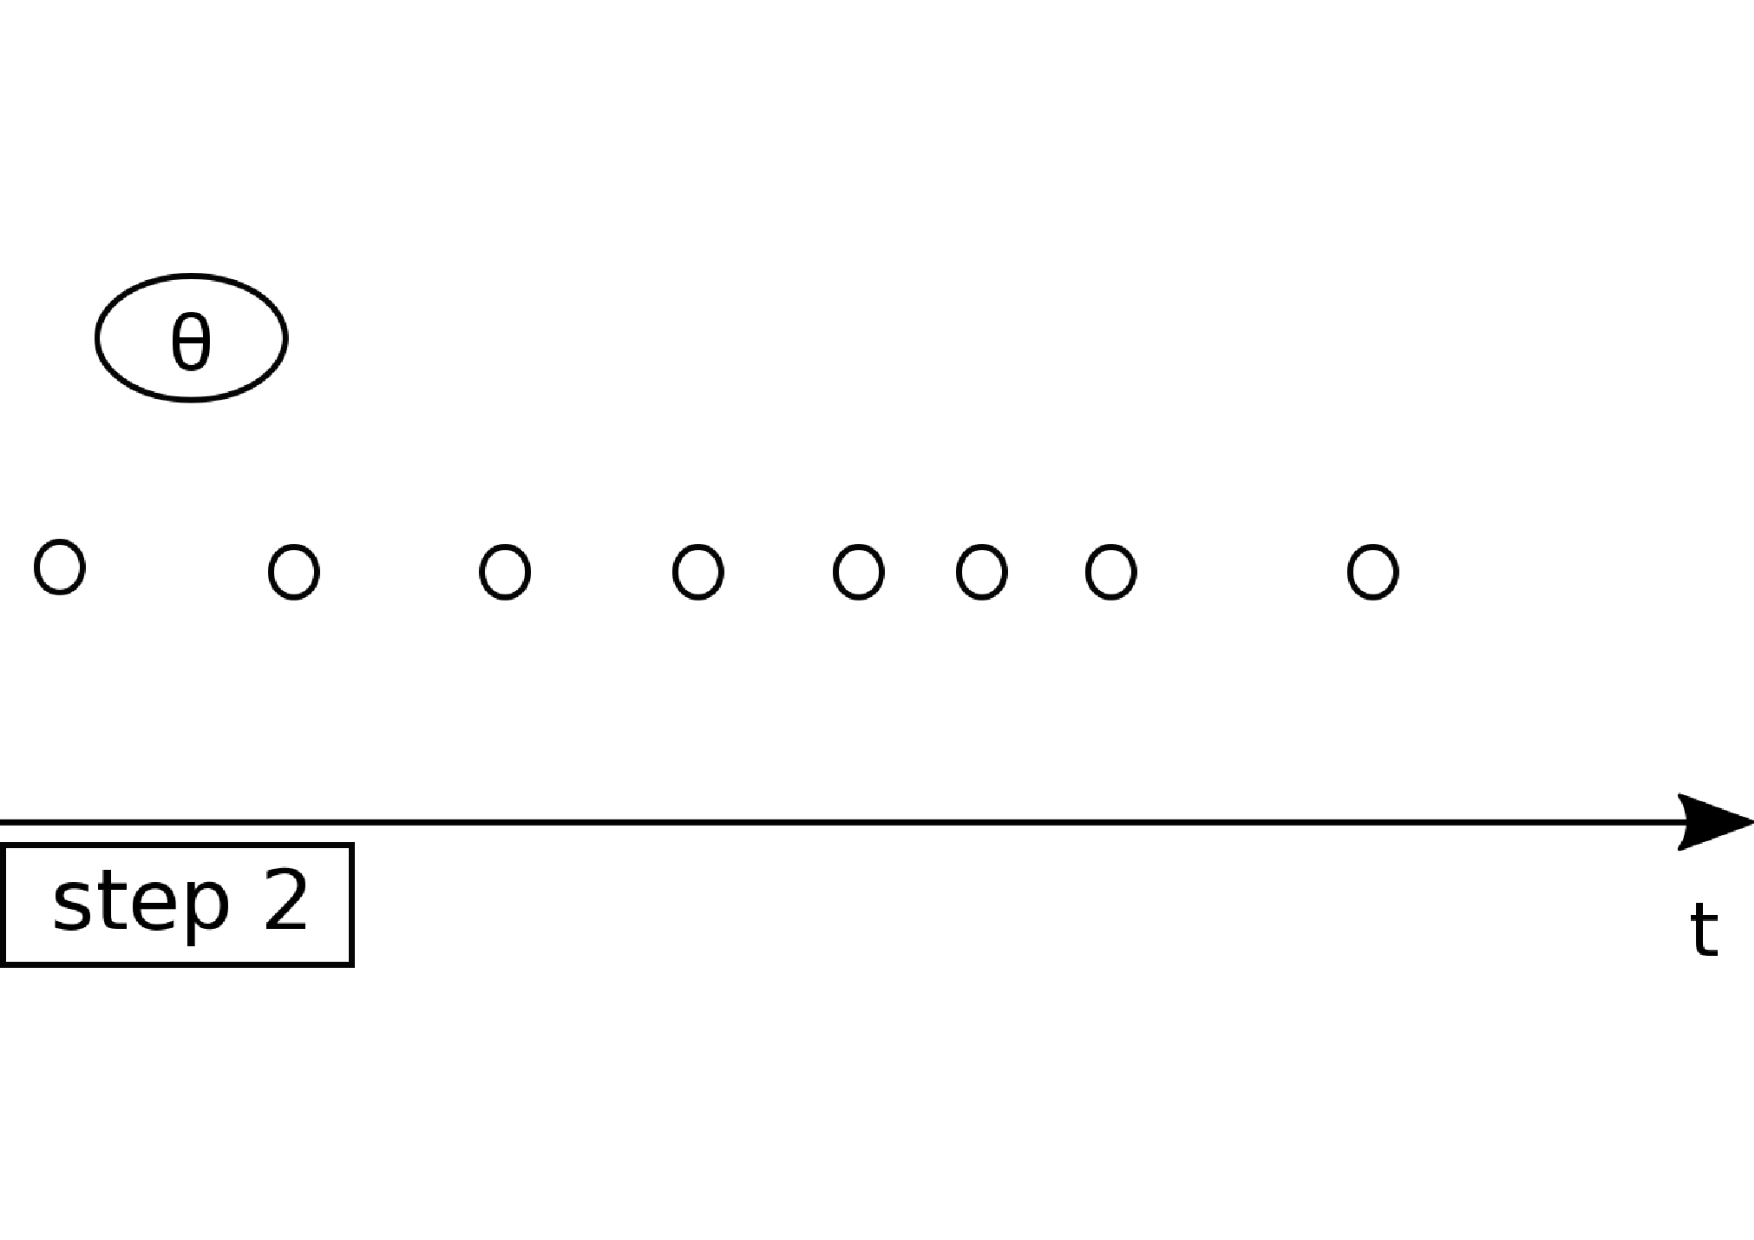
\includegraphics [width=0.70\textwidth, angle=0]{figs/plotn2.pdf}
    \vspace{-0 in}
  \end{minipage}
  \begin{minipage}[!hp]{0.45\linewidth}
  \centering
    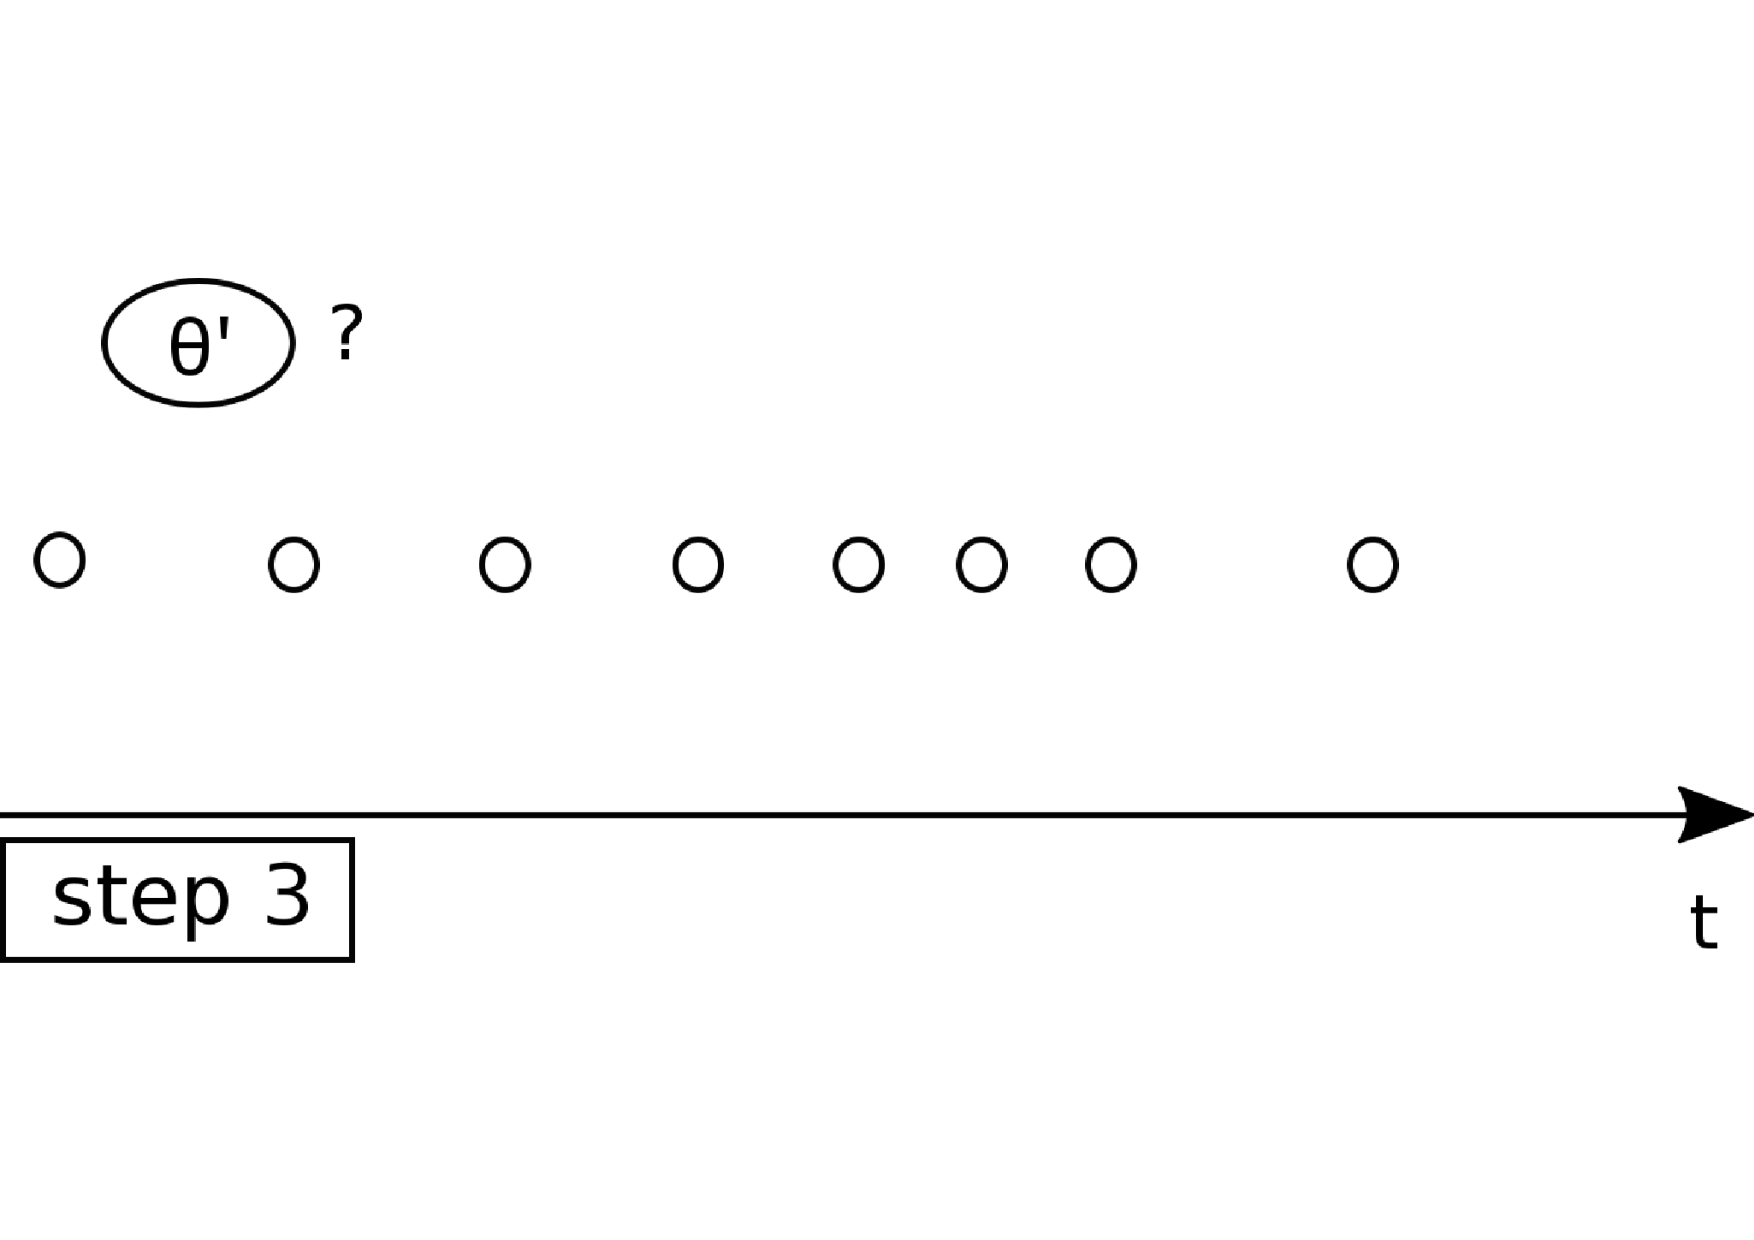
\includegraphics [width=0.70\textwidth, angle=0]{figs/plotn3.pdf}
    \vspace{-0 in}
  \end{minipage}
  \begin{minipage}[!hp]{0.45\linewidth}
  \centering
    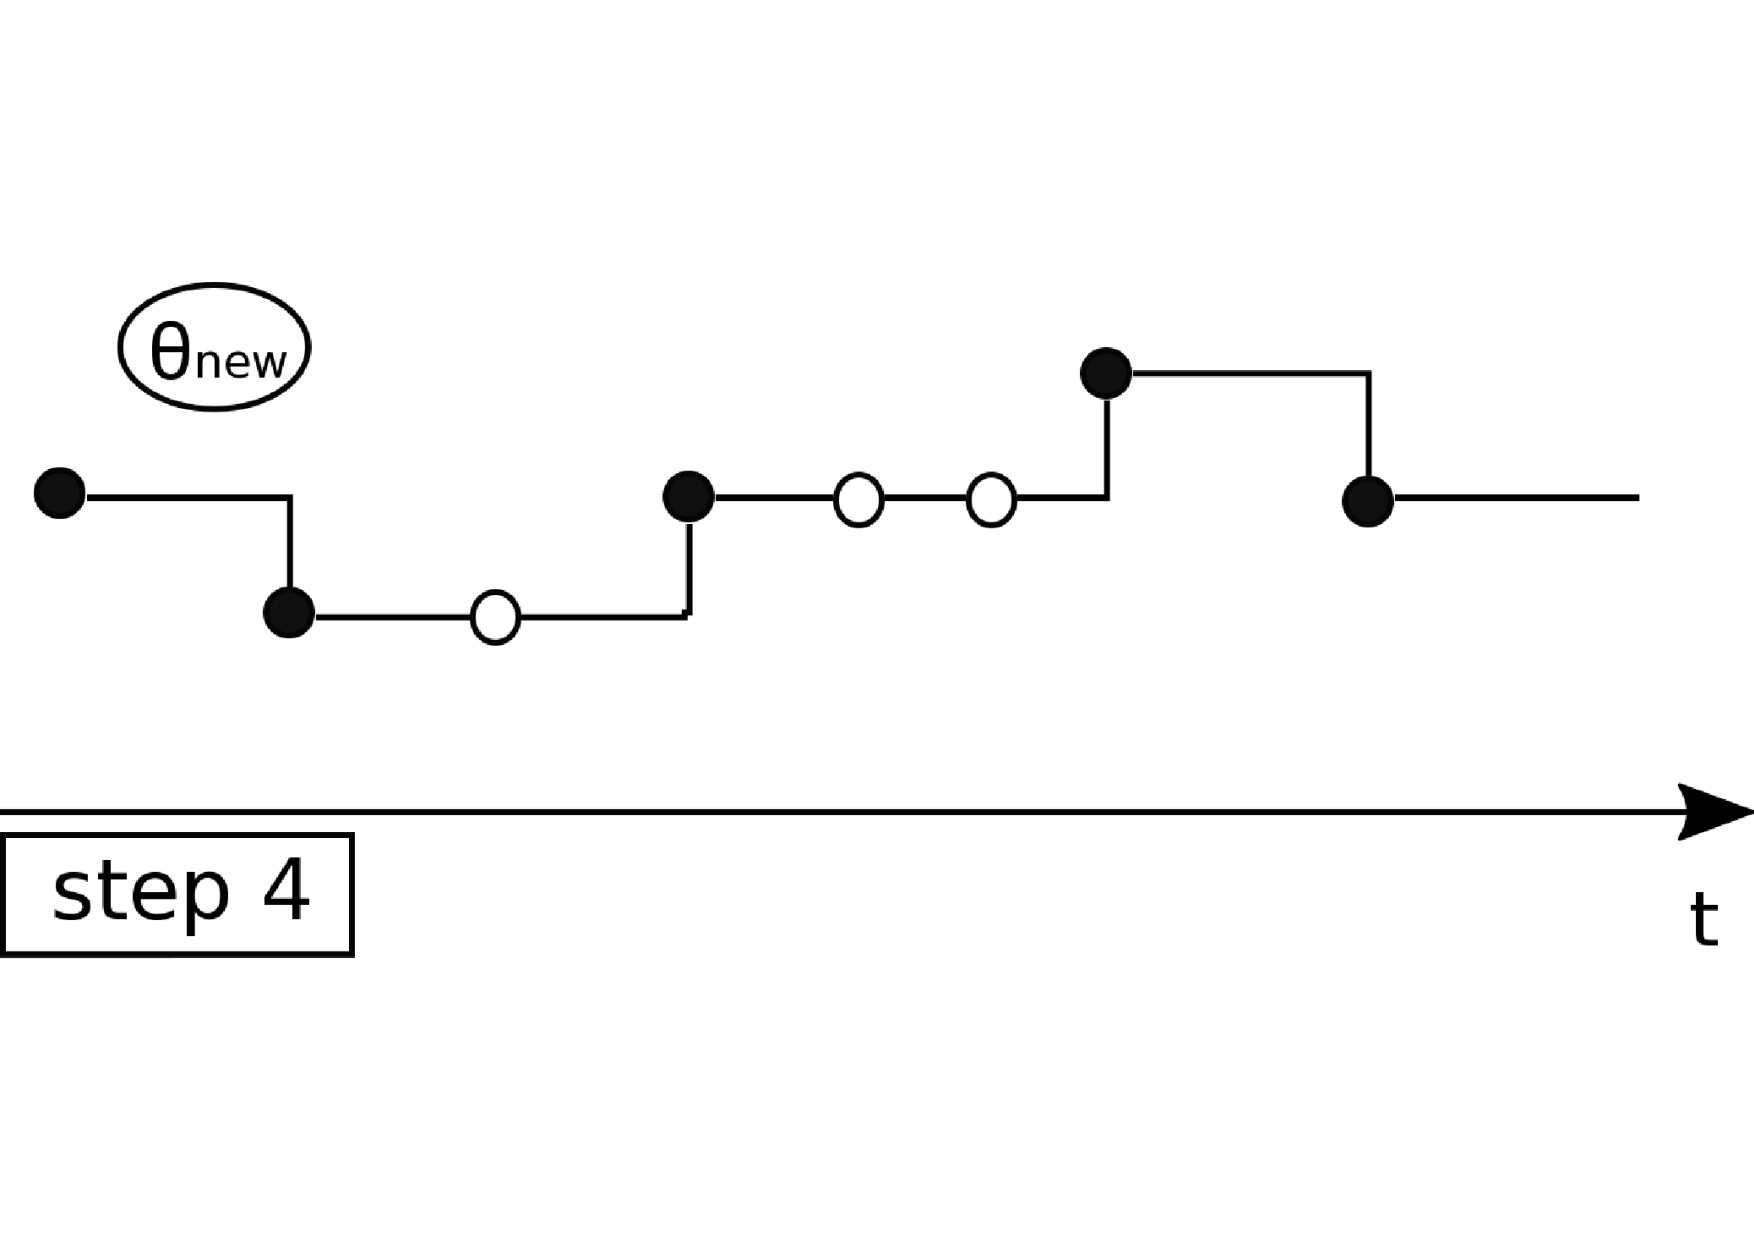
\includegraphics [width=0.70\textwidth, angle=0]{figs/plotn4.pdf}
    \vspace{-0 in}
  \end{minipage}
  \begin{minipage}[!hp]{0.45\linewidth}
  \centering
    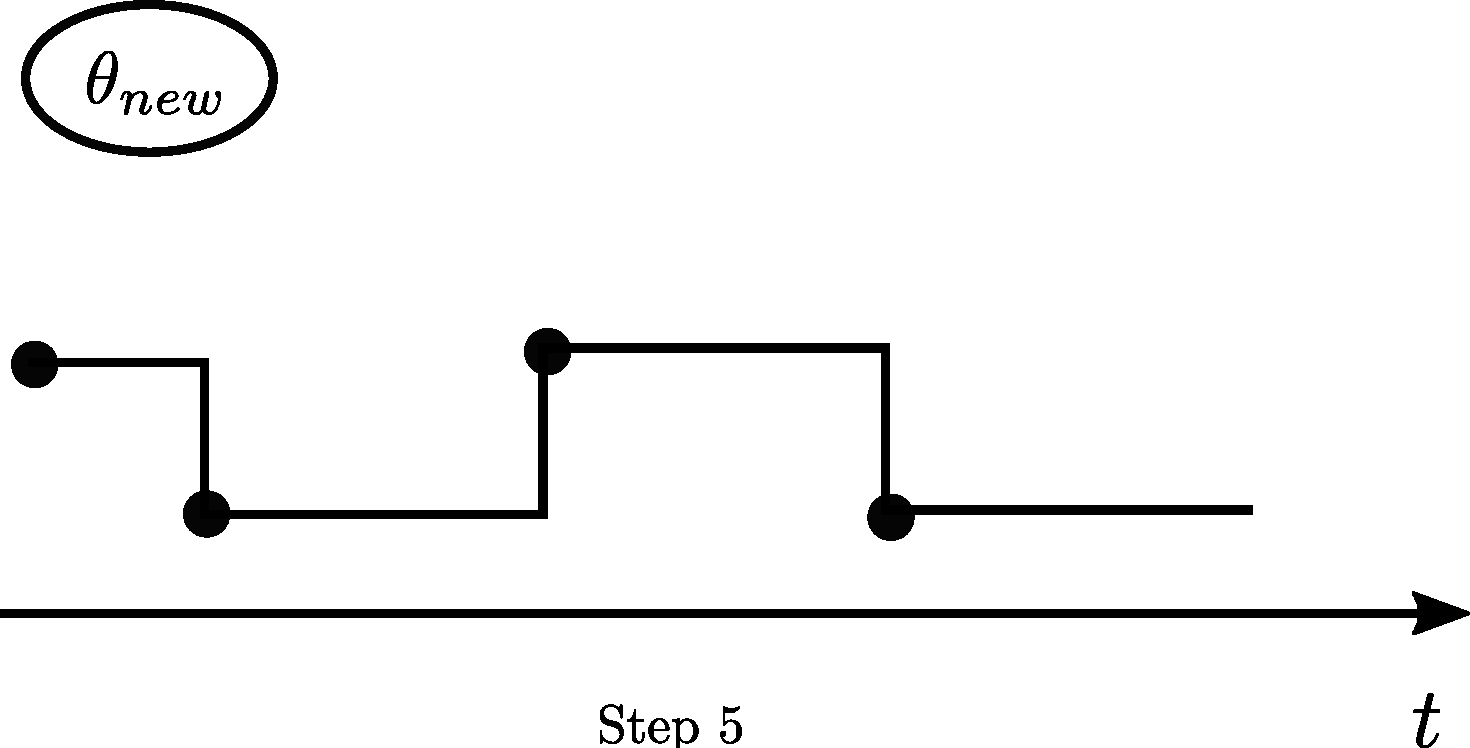
\includegraphics [width=0.70\textwidth, angle=0]{figs/plotn5.pdf}
    \vspace{-0 in}
  \end{minipage}
  \caption{\Naive\ MH-algorithm. Step 0 to 2: sample thinned events
  and discard state information to get a random grid. Step 3: 
propose a new parameter $\theta'$, and accept or reject by making
a forward pass on the grid. Steps 4 to 5: make a backward pass using
the accepted parameter and discard self-transitions to produce a new
trajectory.}
   \label{fig:naive_mh}

  \end{figure}

% \begin{algorithm}[H]
%   \caption{\Naive\ Metropolis-Hastings (MH) sampler for MJP-parameter inference }
%    \label{alg:MH In Gibbs}
% \begin{algorithmic}
%   \State 
%   \begin{tabular}{l l}
%    \textbf{Input:  }  & \text{A set of partial and noisy observations $y_{[t_0, t_{N+1})}$}, \\
%                       & \text{The current MJP path $S(t) = (S, T)$, the current MJP parameters $\theta$}.\\ 
%  \textbf{Output:  }& \text{A new MJP trajectory $\tilde{S} (t) = (\tilde{S}, \tilde{T})$, A series of MJP parameters $\tilde{\theta}$}.
%    \end{tabular}
%    \hrule \\
%     \State 1: Let $\Omega = h(\theta)$, with $\Omega > \max_s{|A_s|}$ using some deterministic function $h$.
%     \State 2: Sample virtual jumps $U\subset[t_{start}, t_{end}]$ from a Non homogeneous Poisson process with piecewise-constant rate$$R(t) = (\Omega + A_{S(t)}).$$\\Define $W = T \cup U$.
%     \State 3: Propose $\theta^* \sim q(.| \theta)$.\\
%         Accept $\theta^*$ as $\tilde{\theta}$ with probability $\alpha$.
%         \begin{align*}
%         \alpha &=  1 \wedge \frac{P(W,\theta^*| y)}{P(W, \theta| y)} \frac{q(\theta|\theta^*)}{q(\theta^*|\theta)}\\
%         &=  1 \wedge \frac{P(y| W,\theta^*) P(W | \theta^*)p(\theta^*)}{P(y|W, \theta)P(W | \theta)p(\theta)} \frac{q(\theta|\theta^*)}{q(\theta^*|\theta)}.
%         \end{align*}
%     \State 4: Sample a path $\tilde{V}$, from a discrete-time Markov chain with $|W| + 1$ steps, using FFBS algorithm. The transition matrix of the Markov chain is $B = (I + \frac{A}{\Omega})$ while the initial distribution over states is $\pi_0$. The likelihood of state $s$ at step $i$ is 
%     $$ L_i(s) = P(Y_{[w_i, w_{i + 1})} | S(t) = s \; for\; t \in [w_i, w_{i + 1})) = \prod_{j: t_j \in [w_i, w_{i + 1})}p(y_{t_j} | S(t_j) = s).$$\\
% %(i.e. $V(i) \sim P(V |  \theta(i), W(i - 1), y).$) Then delete all the virtual jumps to get $S(i), T(i) .$\\
%     \State 5: Let $\tilde{T}$ be the set of times in $W$ when the Markov chain changes state. Define $\tilde{S}$ as the corresponding set of state values. Return $(\tilde{S}, \tilde{T}, \tilde{\theta})$.\\
% \end{algorithmic}
% \end{algorithm}
% \label{sec:meth}

